% !TeX root = ../main.tex
% !TEX root = ../main.tex
% -*- root: ../main.tex -*-
% -*- program: pdflatex -*-
\chapter{喷注味道鉴别流程}
基于机器学习算法设计喷注味道鉴别分类器需要有三个过程,即训练,验证和测试。训练阶段用一部分样本(训练集)对机器学习模型训练,使模型的鉴别能力不断优化提升;验证过程用一部分样本(验证集,不包含训练集)评估训练阶段获得模型的性能,并根据模型在验证集上的性能更改模型超参数,继续进行训练;测试过程用一部分样本(不能包含训练集,测试集)对经过训练,验证过程后的模型进行测试。整个系统主要由四部分组成:数据获取,数据预处理,特征选择和训练,其流程示意图如图~\ref{fig:model_process}~所示。
\begin{figure}[!htb]
  \centering
  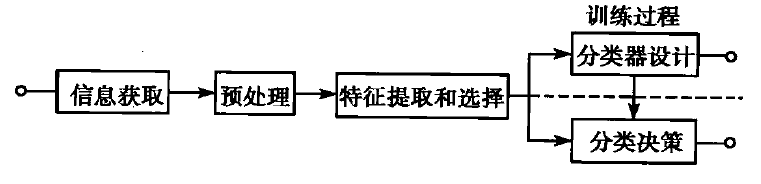
\includegraphics[width=10cm]{chap1/model_process.png}
  \caption{机器学习解决喷注味道鉴别问题流程}
  \label{fig:model_process}
\end{figure}
\section{原始数据获取}
在CEPC实验中,能够被探测装置直接探测到的基本粒子必须满足如下条件:(1).必须是稳定粒子或者有较长的寿命,这样粒子可以在探测器中飞行较长的距离;(2).能够与探测器装置中的物质发生相互作用,因此可以被探测器测量。能够满足上述条件的基本粒子只有有限的几种,常见的有:
$$\gamma,~~ e^{\pm},~~ \mu^{\pm},~~ \pi^{\pm},~~ K^{\pm}, p,~~ \overline{p}.$$
高能物理实验观测到的是上述粒子的响应输出信号,分为时间( TDC )信息和幅度( ADC )信息。CEPC预研阶段,使用Geant4模拟上述信息,将其储存在计算机集群中,以供离线的物理分析。
\section{原始数据预处理}
探测器观测记录的时间信息和幅度信息数据虽然包含了事例的全部可观测信息,但这些信息不能反映事例的”面貌“和性质,不能用来直接作物理分析。将原始数据转化为能够直接反映粒子性质的物理数据过程称为预处理。高能物理的数据预处理包含模拟和重建两个过程。这两个过程在~\cite{zhengzhipeng}中有详细讲解,本文不作介绍。
\section{特征提取和选择}
为了有效地对事例分类识别,需要对预处理后的数据进行筛选和变换,以获得反映事例分类本质特征的物理量,这一过程就是特征提取和选择。特征提取和选择应该有如下三个原则:

(1).有效性,即经过特征提取后的物理量应该能够有效区分信号和本底。

(2).充分性,即提取特征后能够保留事例的完整信息。

(3).具有降维能力,通过特征提取能够有效地减少用它区分信号和本底所需的计算量。

本文